\documentclass{article}

\usepackage{indentfirst}
\usepackage{setspace}
\doublespacing

% ================================================================================= 
% Package for showing source code
% ================================================================================= 

\usepackage{listings}
\usepackage{color}

\definecolor{dkgreen}{rgb}{0,0.6,0}
\definecolor{gray}{rgb}{0.5,0.5,0.5}
\definecolor{mauve}{rgb}{0.58,0,0.82}

\lstset{frame=tb,
language=C,
aboveskip=.5mm,
belowskip=.5mm,
showstringspaces=false,
columns=flexible,
basicstyle={\scriptsize\ttfamily},
numbers=none,
numberstyle=\tiny\color{gray},
keywordstyle=\color{blue},
commentstyle=\color{dkgreen},
stringstyle=\color{mauve},
breaklines=false,
breakatwhitespace=true,
tabsize=3
}

% ================================================================================= 
% Package for flowcharts/diagrams
% ================================================================================= 

\usepackage{tikz}
\usetikzlibrary{shapes.geometric, arrows}

\tikzstyle{startstop} = [rectangle, rounded corners, minimum width=3cm, minimum height=1cm,text centered, draw=black, fill=red!30]
\tikzstyle{io}        = [rectangle, minimum width=3cm, minimum height=1cm,text centered, draw=black, fill=blue!30]
\tikzstyle{process}   = [diamond, minimum width=2cm, minimum height=0cm, text centered, draw=black, fill=orange!30]
\tikzstyle{arrow}     = [thick,->,>=stealth]

% ==================================================
% Paper
% ==================================================

\title{Fully Generalized Compilation}
\date{01-26-2017}
\author{Lucas Saldyt}

\begin{document}

\maketitle
\pagenumbering{gobble}
\newpage
\pagenumbering{arabic}

% ==================================================
\section{Abstract}
% ==================================================

Assuming that two languages are \textit{isomorphic}, one language can be converted to another if given an adequate description of each language's grammar.
At an abstract level, this conversion is entirely practical. However, in practice,  
Progtran is an investigation into the feasibility of a \textbf{Fully Generalized Compiler}, a multi-language source-to-source compiler. 
Given source code in one language, a description of its grammar \textbf{A} , and a description of an output language's grammar \textbf{B}, can \textbf{A} be converted to \textbf{B} such that the output in \textbf{B} is indistinguishable from a program originally written in \textbf{B}?

% ==================================================
\section{Introduction}
% ==================================================

A \textbf{Full Generalized Compiler} is a tool for programming language researchers, providing a \textit{dynamic framework} for easily modifying syntax of input and output languages. 
A new programming language can even be fully implemented without recompiling the software. 
Progtran also uses this concept (user defined dynamic grammars) to re-implement existing source-to-source compilation tools, such as \textbf{Cython} or \textbf{2to3}.

% ==================================================
\section{Methods}
% ==================================================

\subsection{Traditional Compilation}
Brief description of how compilers work

\subsection{Abstracting Language Definitions}
Description of grammar, transformation, and constructor files

\subsection{Grammars}
Influence of formal grammars

Description of grammar file implementations 

\subsection{AST Transformations}

Reasoning for and description of AST-transformations

\subsection{Constructors}

Description of Constructor implementation

\subsection{Compilation in Glossa}
Given all of the above details, how does compilation in Glossa compare to the traditional compilation process?

(Grammar/Transform/Construction rules are read at run-time)

\newpage

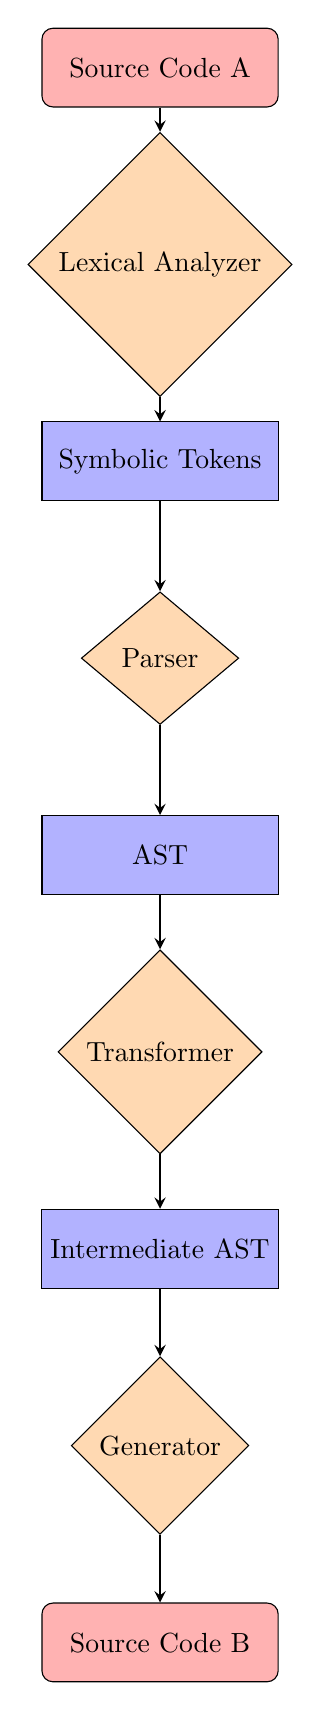
\begin{tikzpicture}[node distance=2.5cm]

    \node (sourcea) [startstop]                 {Source Code A};
    \node (lexer)   [process, below of=sourcea] {Lexical Analyzer};
    \node (tokens)  [io, below of=lexer]        {Symbolic Tokens};
    \node (parser)  [process, below of=tokens]  {Parser};
    \node (asta)    [io, below of=parser]       {AST};
    \node (trans)   [process, below of=asta]    {Transformer};
    \node (astb)    [io, below of=trans]        {Intermediate AST};
    \node (gen)     [process, below of=astb]    {Generator};
    \node (stop)    [startstop, below of=gen]   {Source Code B};


    \draw [arrow] (sourcea) -- (lexer);
    \draw [arrow] (lexer) -- (tokens);
    \draw [arrow] (tokens) -- (parser);
    \draw [arrow] (parser) -- (asta);
    \draw [arrow] (asta) -- (trans);
    \draw [arrow] (trans) -- (astb);
    \draw [arrow] (astb) -- (gen);
    \draw [arrow] (gen) -- (stop);

\end{tikzpicture}


% ==================================================
\section{Applications}
% ==================================================

\subsection{Re-implementation of Cython and 2to3}
Description of implementing these two pieces of software with glossa

\subsection{Cython}
\subsection{2to3}

\subsection{Comparisons and Benchmarks}

\subsection{Simple code porting}
Reference work on 2to3, talk about FORTRAN and similar conversions

\subsection{Language Creation}
Description of implementing new programming languages using glossa

\subsection{Language Design and Modification}
\subsection{Glossa as a pre-processor}

% ==================================================
\section{Results}
% ==================================================

\subsection{Results Overview}

2to3 comparison

Cython comparison

GHC comparison

\subsection{Quicksort Cython Comparison}

This is not meant to be a robust benchmark. Instead, it aims to show that Cython and Transpilation yield similar results.

Output for 1000 sorting iterations:
\begin{center}
    \begin{verbatim}
        Transpile speedup:
        13.335545461765733
        Cython speedup:
        13.9866371311344
        Transpile : Cython comparison 
        0.9534
    \end{verbatim}
\end{center}

\newpage
\subsection{Original Python Code}

\lstset{language=Python}
\begin{lstlisting}
def sort(array):
    less    = []
    equal   = []
    greater = []

    if len(array) <= 1:
        return array
    else:
        pivot = array[0]
        for x in array:
            if x < pivot:
                less.append(x)
            if x == pivot:
                equal.append(x)
            if x > pivot:
                greater.append(x)
        return sort(less) + equal + sort(greater)

def main():
    l = sort([3, 2, 12, 9, 4, 68, 17, 1, 2, 3, 4, 5, 6, 12, 9  , 8, 7, 6,5, 4, 743])

if __name__ == "__main__":
    main()
\end{lstlisting}

\lstset{language=C}

\newpage
\subsection{Generated C++ Code (Glossa)}

\begin{lstlisting}
#include "../std/std.hpp"
template <typename T_array>
auto sort (T_array array)
{
    auto less = std::vector<Object>({});
    auto equal = std::vector<Object>({});
    auto greater = std::vector<Object>({});
    if (len(array) <= 1)
    {
        return array;
    }
    else
    {
        auto pivot = array[0];
        for (auto x : array)
        {
            if (x < pivot)
            {
                less.push_back(x);
            }
            if (x == pivot)
            {
                equal.push_back(x);
            }
            if (x > pivot)
            {
                greater.push_back(x);
            }
        };
        return sort(less) + equal + sort(greater);
    };
}
\end{lstlisting}

\newpage
\subsection{Generated C Code (Cython)}

Generated code for Cython is much more complex, as it integrates with the Python FFI

For example, this snippet declares an empty array

\begin{lstlisting}
  /* "main.py":6
 *     Sorts an array of comparable values
 *     """
 *     less    = []             # <<<<<<<<<<<<<<
 *     equal   = []
 *     greater = []
 */
  __pyx_t_1 = PyList_New(0); if (unlikely(!__pyx_t_1)) {__pyx_filename = __pyx_f[0]; __pyx_lineno = 6; __pyx_clineno = __LINE__; goto __pyx_L1_error;}
  __Pyx_GOTREF(__pyx_t_1);
  __pyx_v_less = ((PyObject*)__pyx_t_1);
  __pyx_t_1 = 0;
\end{lstlisting}

\newpage

% ==================================================
\section{Conclusion}
% ==================================================


\end{document}
